\subsection{To-do list} \setclass{ToDoList} \label{\class}
\begin{figure}[H]
	\centering
	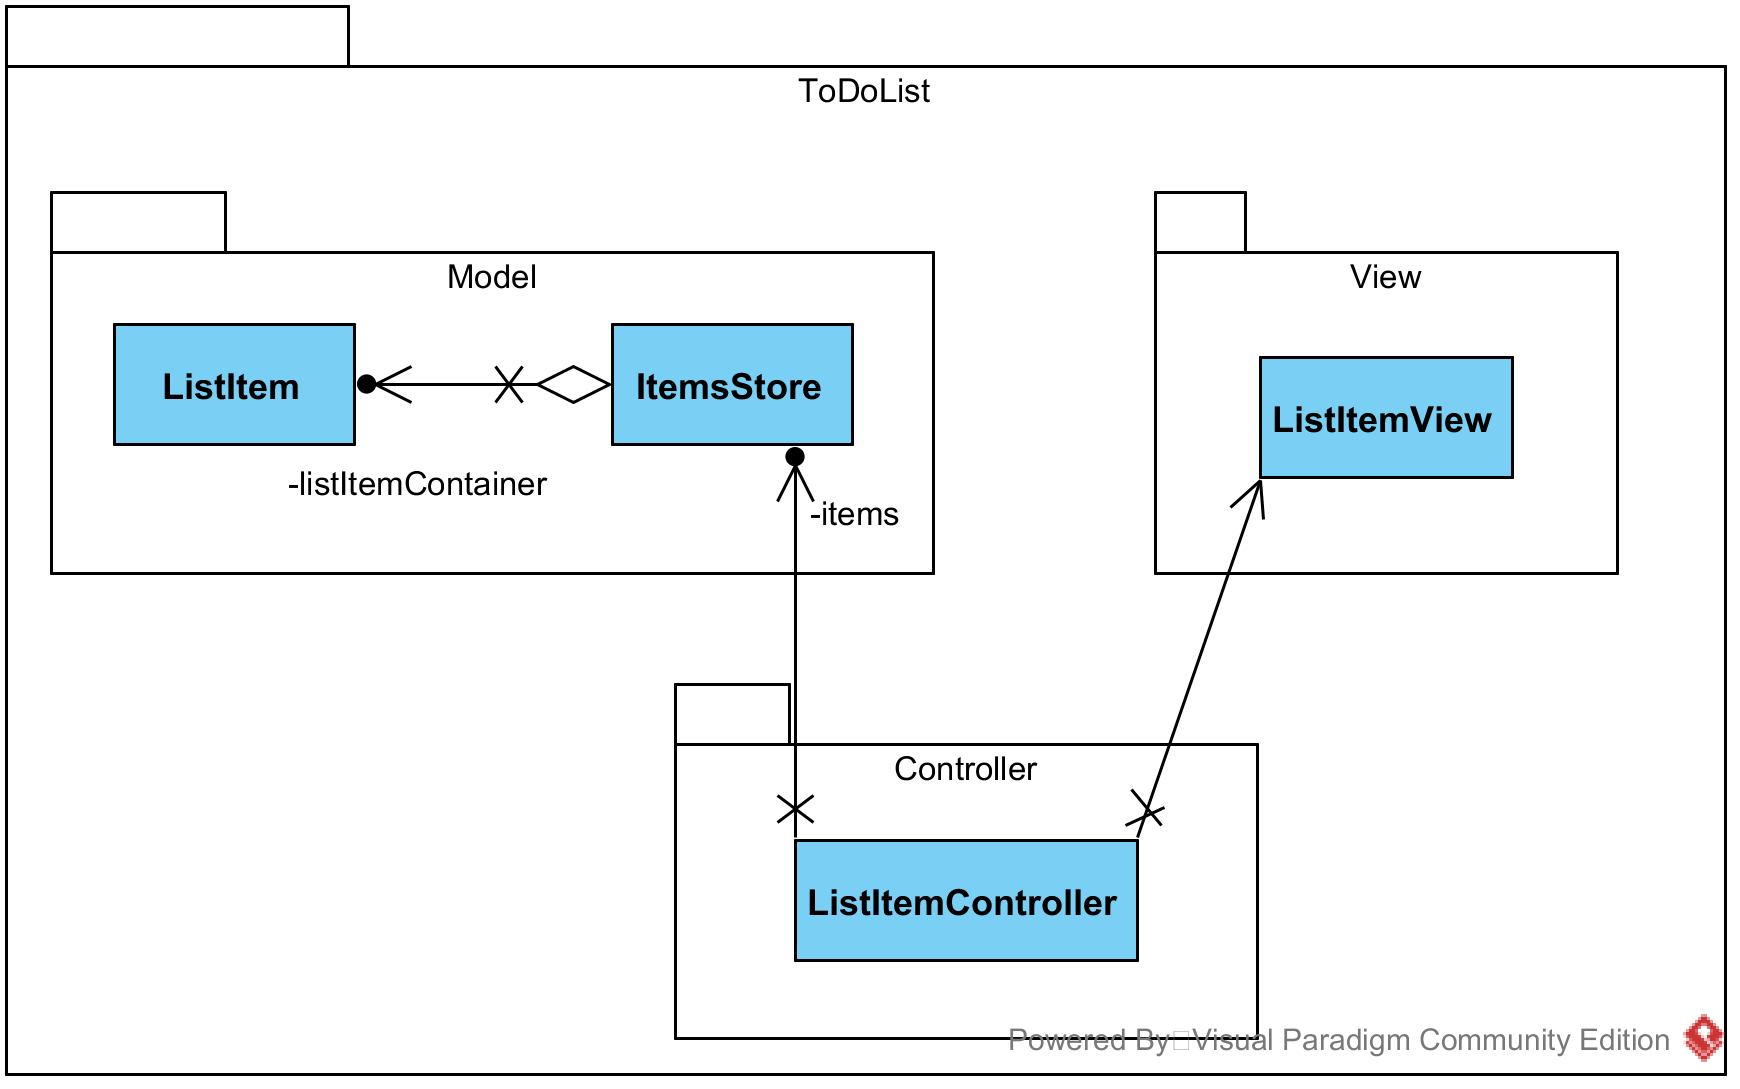
\includegraphics[width=14cm]{./diagrammi/todo/todo.png}
	\caption{Componente ToDoList}
\end{figure}
\glossario{TodoList} è il package base per la prima delle due demo. Come il framework segue il design pattern MVC ed è quindi composto dai package Model, View e Controller.

\setclass{ToDoList::Model}
\subsubsection[::Model]{\class} \label{\class}
\begin{figure}[H]
	\centering
	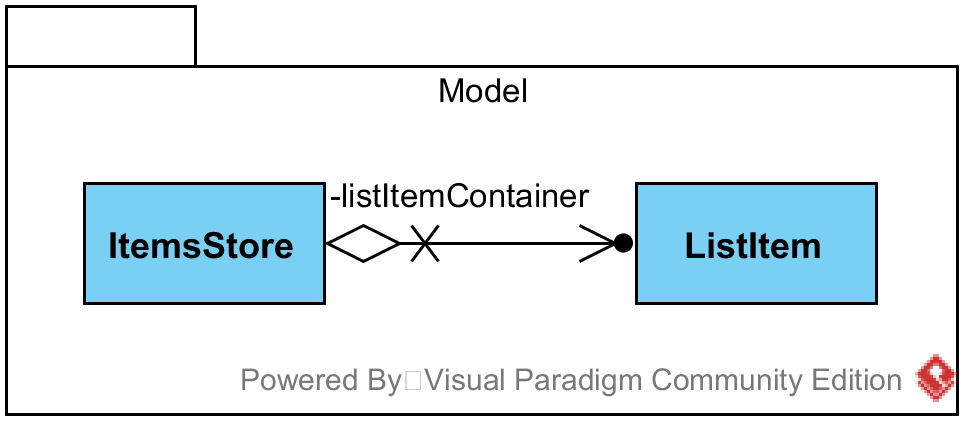
\includegraphics[width=10cm]{./diagrammi/todo/todomodel.png}
	\caption{Componente \class}
\end{figure}
Il package Model gestisce i dati della To-do list ed è composto a sua volta dalle classi ItemsStore e ListItem.


\setclass{TodoList::Model::ItemsStore}
\paragraph[::ItemsStore]{\class}\mbox{}\\ \label{\class}
\begin{figure}[H]
	\centering
	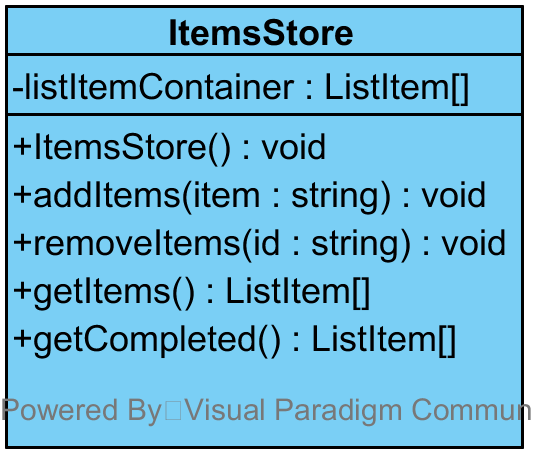
\includegraphics[width=7cm]{./diagrammi/todo/itemsstore.png}
	\caption{Classe \class}
\end{figure}
\textbf{Descrizione:}
ItemsStore implementa la classe BubbleMemory e gestisce i dati della To-do list.

\textbf{Utilizzo:}
Viene utilizzata per gestire gli elementi della To-do list.

\textbf{Classi ereditate:}
\begin{itemize}
	\item \coderef{Framework::Model::BubbleMemory::BubbleMemory}.
\end{itemize}

\textbf{Attributi:}
\begin{itemize}
	\item \field{- listItemContainer: ListItem[]}: array contenente gli elementi della lista;
\end{itemize}

\textbf{Metodi:}
\begin{itemize}
	\item \method{+ ItemsStore(): void}: costruttore della classe, crea l'array vuoto degli elementi della lista;
	\item \method{+ addItems(item: string): void}: aggiunge un elemento alla lista;
	\begin{itemize}
		\item \param{item: string}: nome dell'elemento da aggiungere alla lista.
	\end{itemize}
	\item \method{+ removeItems(id: string): void}: rimuove l'elemento identificato da id dalla lista;
	\begin{itemize}
		\item \param{id: string}: id dell'oggetto da rimuovere.
	\end{itemize}
	\item \method{+ completeItems(id: string): void}: indica come completato l'elemento id;
	\begin{itemize}
		\item \param{id: string}: id dell'oggetto da indicare come completato.
	\end{itemize}
	\item \method{+ getItems(): ListItem[]}: restituisce tutti gli elementi della lista;
	\item \method{+ getCompleted(): ListItem[]}: restituisce tutti gli elementi completati della lista;
\end{itemize}

\setclass{TodoList::Model::ListItem}
\paragraph[::ListItem]{\class}\mbox{}\\ \label{\class}
\begin{figure}[H]
	\centering
	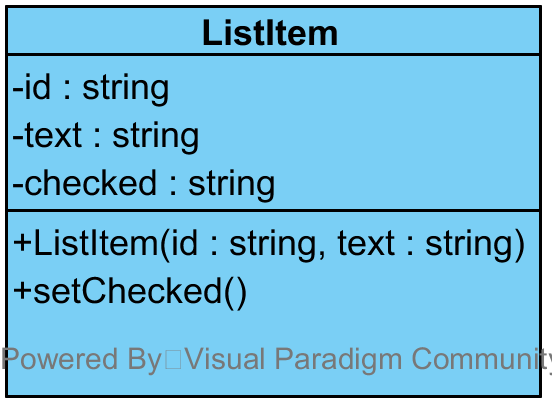
\includegraphics[width=7cm]{./diagrammi/todo/todolistitem.png}
	\caption{Classe \class}
\end{figure}
\textbf{Descrizione:}
ListItem rappresenta un singolo elemento della lista To-do list.

\textbf{Utilizzo:}
Viene utilizzata per rappresentare gli elementi della To-do list.

\textbf{Attributi:}
\begin{itemize}
	\item \field{- id: string}: id unico identificativo dell'elemento;
	\item \field{- text: string}: testo dell'elemento;
	\item \field{- checked: bool}: stato dell'elemento: 
	\begin{itemize}
		\item true: completato;
		\item false: non completato.
	\end{itemize}
\end{itemize}

\textbf{Metodi:}
\begin{itemize}
	\item \method{+ ListItem(id: string, text: string)}: costruttore della classe;
	\begin{itemize}
		\item \param{id: string}: input dell'identificativo unico dell'elemento;
		\item \param{text: string}: testo dell'elemento;
	\end{itemize}
	\item \method{+ setChecked ()}: modifica lo stato dell'elemento per indicarlo come completato.
\end{itemize}

\setclass{TodoList::View}
\subsubsection[::View]{\class} \label{\class}
Il package View si occupa di gestire la parte grafica della To-do list, ed è composto dalla classe ListItemView.

\setclass{TodoList::View::ListItemView}
\paragraph[::ListItemView]{\class}\mbox{}\\ \label{\class}
\begin{figure}[H]
	\centering
	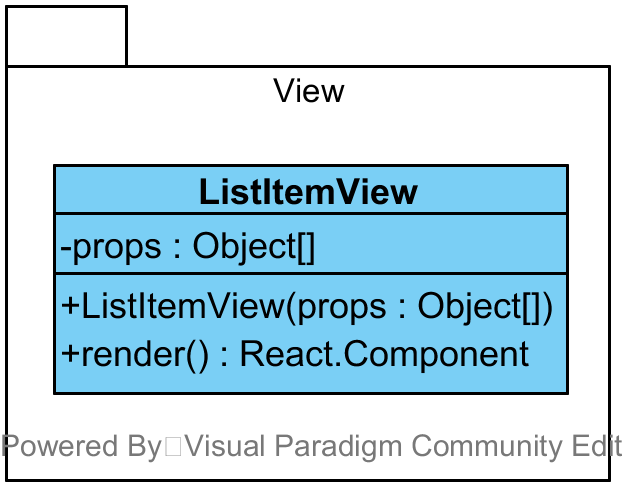
\includegraphics[width=7cm]{./diagrammi/todo/todoview.png}
	\caption{Classe \class}
\end{figure}
\textbf{Descrizione:}
Questa classe gestisce la visualizzazione degli elementi della To-do list.

\textbf{Utilizzo:}
Viene utilizzata per gestire la view della To-do list.

\textbf{Classi ereditate:}
\begin{itemize}
	\item \code{React::Component}.
\end{itemize}

\textbf{Attributi:}
\begin{itemize}
	\item \field{- props: Object[]}: array contenente le proprietà degli elementi della lista.
\end{itemize}

\textbf{Metodi:}
\begin{itemize}
	\item \method{+ ListItem(props: Object[])}: costruttore della classe, assegna le proprietà:
	\begin{itemize}
		\item \param{props: Object[]}: array contenente le proprietà degli elementi.
	\end{itemize}
	\item \method{+ render(): React::Component}: renderizza il componente.
\end{itemize}

\setclass{TodoList::Controller}
\subsubsection[::Controller]{\class} \label{\class}
Il package controller è composto dalla classe ListItemController.


\setclass{TodoList::Controller::ListItemController}
\paragraph[::ListItemController]{\class}\mbox{}\\ \label{\class}
\begin{figure}[H]
	\centering
	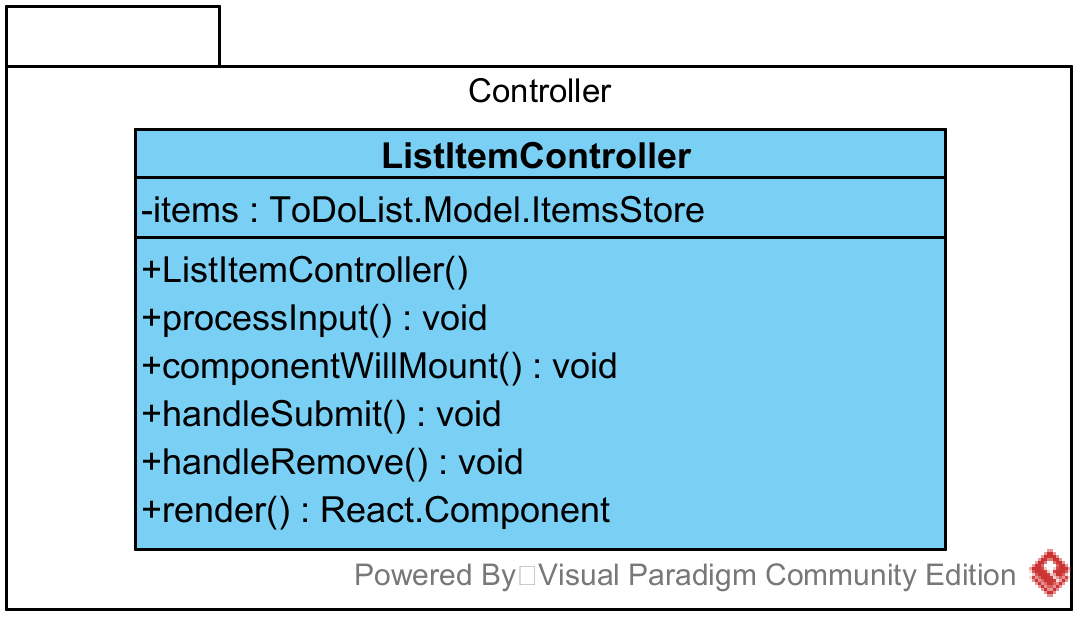
\includegraphics[width=10cm]{./diagrammi/todo/todocontroller.png}
	\caption{Classe \class}
\end{figure}
\textbf{Descrizione:}
Questa classe rappresenta il controller della To-do list.

\textbf{Utilizzo:}
Viene utilizzata per associare agli elementi della view le funzionalità logiche rese disponibili dal model.

\textbf{Classi ereditate:}
\begin{itemize}
	\item \code{React::Component};
\end{itemize}

\textbf{Attributi:}
\begin{itemize}
	\item \field{- items: ItemStore}: store di salvataggio della lista;
\end{itemize}

\textbf{Metodi:}
\begin{itemize}
	\item \method{+ ListItemController()}: costruttore della classe, crea lo store di salvataggio della lista;
	\item \method{+ processInput(): void}: costruisce la lista di ListItem;
	\item \method{+ componentWillMount(): void}: recupera i dati dal model alla creazione della classe;
	\item \method{+ handleComplete(): void}: comunica al model di completare un elemento della lista;
	\item \method{+ handleSubmit(): void}: comunica al model di aggiungere un elemento alla lista;
	\item \method{+ handleRemove(): void}: comunica al model di rimuovere un elemento dalla lista;
	\item \method{+ render(): React::Component}: renderizza il componente.
\end{itemize}
